% !TeX spellcheck = ru_RU
% !TEX root = vkr.tex

\section{Обзор tokio}

Настоящая глава содержит описание реализации многопоточного рантайма tokio, асинхронного интерфейса языка Rust. К сожалению, \verb|tokio| не имеет архитектурной документации, а работы~\cite{cringeTokioIOUring} связанные с исследованием \verb|tokio| не многочислены и не содержательны, поэтому данная глава призвана создать представление об устройстве планировщика многопоточного рантайма для последующего исследования его производительности.

\subsection{Планировщик многопоточного рантайма tokio}

При создании рантайм создает определенное количество системных потоков для так называемого блокирующего пулла, призванного исполнять ресурсоемкие задачи. Всего создается \verb|worker_threads| + \verb|max_blocking_threads| потоков, где

\begin{itemize}
    \item \verb|worker_threads| --- количество потоков, предназначенных для исполнения асинхронных задач
    \item \verb|max_blocking_threads| --- максимальное количество блокирующих потоков
\end{itemize}

\begin{figure}[H]
    \begin{center}
        \makebox[\textwidth]{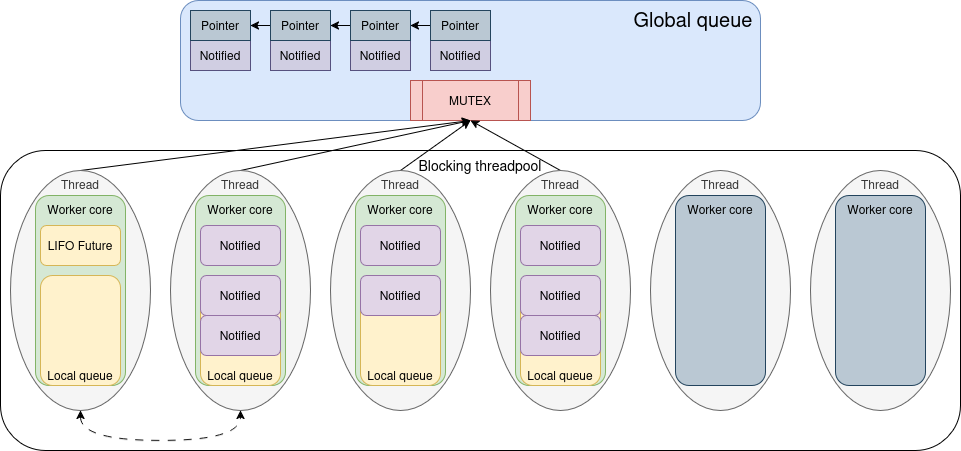
\includegraphics[scale=0.55]{pictures/tokio_arch.drawio.png}}
    \end{center}

    \caption{Упрощенное представление многопоточного рантайма.}
    \label{fig:tokio:arch}
\end{figure}

\verb|Notified| --- тип единицы планирования в tokio. Далее в тексте они также будут называться задачами.

\verb|Исполнитель|, так называется сущность исполняющая задачи. Она ассоциированна с каждым из \verb|worker_threads| потоков с помощью размещения в локальной для этих потоков переменной так называемого \verb|ядра исполнителя| --- структуры, необходимой для исполнения асинхронных задач, включающей \verb|локальную очередь|, указатель \verb|глобальной очереди| и тому подобное.

\verb|Локальная очередь| исполнителя выступает в качестве кэша задач, имеет фиксированный размер и предполагает добавление элементов  исключительно из потока владельца. Однако, изъятие из нее может быть осуществлено потоками других исполнителей при нехватке задач --- процесс называемый похищением~\cite{cringeTokioIOUring}. Все это: фиксированный размер и производитель в единственном количестве --- позволяет ей иметь lock free реализцию. В случае переполнения часть элементов перемещается в глобальную очередь.

\verb|Глобальная очередь| или \verb|InjectedQueue| представляет собой очередь произвольного размера для агрегации задач. Реализована с помощью интрузивного связного списка~\cite{queues}, защищенного мьютексом. Именно этот ресурс по мнению разрабочиков из YADRO ограничивает пропускную способность рантайма.

В рамках данной работы будет рассмотрен единственный метод интерфейса планировщика --- \verb|schedule_task()|. Именно он используется для отправления на исполнение в планировщик задач. Большое значение имеет контекст вызова этого метода:

\begin{itemize}
    \item В потоке исполнителя задача будет помещена в его локальную очередь.
    \item В ином случае, задача будет помещена в \verb|InjectedQueue|.
\end{itemize}

\subsection{Асинхроное замыкание}

На листинге~\ref{listing:async_closure} представлен код демонстрирующий описание асинхронного замыкания в языке \verb|Rust|.

\begin{listing}[H]
    \begin{minted}{rust}
async {}
    \end{minted}

    \caption{Асинхронное замыкание.}
    \label{listing:async_closure}
\end{listing}

Значениие связанное с именем \verb|closure| представляет собой конечный автомат, сгенерированный компилятором, автоматически реализующий интерфейс, представленный на листинге~\ref{listing:future_trait}.

\begin{listing}[H]
    \begin{minted}{rust}
trait Future {
    type Output;
    fn poll(self: Pin<&mut Self>, cx: &mut Context)
        -> Poll<Self::Output>;
}
    \end{minted}

    \caption{Интерфейс асинхронных конечных автоматов в языке Rust.}
    \label{listing:future_trait}
\end{listing}

Где метод \verb|poll()| выражает попытку совершить переход от состояния к состоянию и сигнализиует о завершении выполнения замыкания с помощью возвращаемого значения типа представленного на листинге~\ref{listing:future:poll}.

\begin{listing}[H]
    \begin{minted}{rust}
enum Poll<T> { Ready(T), Pending }
    \end{minted}

    \caption{Асинхронное замыкание.}
    \label{listing:future:poll}
\end{listing}

Способного представить результирующее значение асинхронного вычисления в варианте \verb|Ready| или сигнализировать об отсутствии готового результата с вариантом \verb|Pending|.

Метод \verb|poll()| в качестве первого аргумента принимает само асинхронное замыкание, окруженное структурой \verb|Pin|, --- это необходимо для статической гарантии безопасности. В качестве второго аргумента --- контекст, служащий оберткой для значния \verb|Waker|.

\subsection{Waker}

Типичным сценарием использования значения \verb|Waker| является:

\begin{itemize}
    \item Создание с помощью специфичной для рантайма таблицы виртуальных методов.
    \item Передача в метод \verb|poll()| внутри структуры \verb|Context|.
    \item Если метод \verb|poll()| вернул \verb|Pending| --- замыкание должно зависящим от реализации способом сохранить \verb|Waker| для вызова его метода \verb|wake()| при готовности совешать прогресс.
\end{itemize}

То есть \verb|Waker| является связующим звеном между асинхронным ресурсом и исполнителем асинхронных замыканий, сообщающим первому о готовности второго.

\begin{itemize}
    \item Асинхронный ресурс --- листовое асинхронное замыкание, реализованное библиотекой tokio, абстрагирующее архитектурно зависимые интерфейсы, например: \verb|epoll|~\cite{epollLib}, \verb|kqueue|~\cite{kqueue}.
    \item Исполнитель асинхронных замыканий --- в случае tokio планировщик.
\end{itemize}

\subsection{Интерфейс tokio}

Вследствие выше сказанного любое асинхронное замыкание можно исполнить достаточно долго вызывая на нем метод \verb|poll()|, передавая в него \verb|Waker| --- пустышку. Однако, для удобства и эффективности использования асинхронного интерфейса, предоставляемого языком \verb|Rust|, проект \verb|tokio| предлагает собственный интерфейс для исполнения асинхронных замыканий.

\subsubsection{tokio::spawn()}

Метод \verb|tokio::spawn()|, регистрирующий асинхронное замыкание на исполнение в рантайме \verb|tokio|, возвращает значение \verb|JoinHandle|, позволяющее ожидать исполнения исходного замыкания, получать результирующее значение или отменять исполнение вовсе. Например, исполнить представленное выше замыкание можно способом, приведенным на листинге~\ref{listing:tokio_spawn::sleep}:

\begin{listing}[H]
    \begin{minted}{rust}
let join: JoinHandle<()> = tokio::spawn(async {});
    \end{minted}

    \caption{Пример исполнения замыкания с помощью tokio.}
    \label{listing:tokio_spawn::sleep}
\end{listing}

Где пользователь аллоцирует замыкание в \verb|tokio| рантайме передавая его в метод \verb|tokio::spawn()|.

\subsubsection{tokio::yield\_now()}

Метод \verb|tokio::task::yeild_now()| предоставляет возможность вернуть поток управления планировщику, тем самым создав еще одно состояние в конечном автомате асинхронного замыкания. Его использование приведено на листинге~\ref{listing:tokio_yield_now}.

\begin{listing}[H]
    \begin{minted}{rust}
async { task::yield_now().await }
    \end{minted}

    \caption{Пример возвращение управления планировщику в tokio.}
    \label{listing:tokio_yield_now}
\end{listing}

При исполнении \verb|yield_now()| вернет управление исполнителю замыкания, тем самым не позволит выполнить себя за один вызова метод \verb|poll()|.

\verb|yield_now| является листовым асинхронным замыканием, однако, никакого настоящего ресурса под собой не содержит. То есть отсутствует внешняя сущность, способная уведомить рантайм о готовности замыкания продолжать вычисления --- некому хранить \verb|Waker|. В подобных случаях для сохранения инстансов типа \verb|Waker| используется, локальная для потока исполнителя, коллекция, куда помещается структура \verb|Waker|.

\subsection{Жизненный цикл асинхронного замыкания}

В данном разделе буде описан процесс аллокации асинхронного замыкания и создания первой \verb|Notified| для него.

\subsubsection{Аллокация асинхронного замыкания}

Обработка асинхронного замыкания переданного пользователем в метод \verb|tokio::spawn()| содержит следующие шаги:

\begin{itemize}
    \item Создание уникального индентификатора. Происходит это с помощью статической атомарной переменной, над которой выполняется FAA с relaxed семантикой.
    \item Аллокация структуры, содержащей замыкание, счетчик указателей и слот для результирующего значения, --- так называемой \verb|Cell| на куче.
    \item Создание трех указателей на эту область памяти: \verb|Task|, \verb|Notified| и \verb|JoinHandle|.
    \begin{itemize}
        \item \verb|Task| помещается в \verb|OwnedTasks| --- очередь, предназначенную для хранения указателей на все замыкания, исполняемые рантаймом.
        \item \verb|Notified| отправляется в планировщик c помощью метода \verb|schedule_task()|.
        \item \verb|JoinHandle| возвращается пользователю.
    \end{itemize}
\end{itemize}

\subsubsection{Исполнение замыкания}

Далее, происходит исполнение замыкания: после вызова метода \verb|wake()| у соотвествующего инстанса типа \verb|Waker|, новый указатель \verb|Notified| отправляется в планировщик \verb|tokio| рантайма c помощью метода \verb|schedule_task()|. Далее у \verb|Notified| будет вызван метод \verb|poll()|, что повлечет исполнение метода \verb|poll()| на исходном замыкании.

Таким образом по готовности каждого асинхронного замыкания уже аллоцированного \verb|tokio| рантаймом создается указатель \verb|Notified|, отправляемый на исполнение в планировщик с \verb|schedule_task()|.

\subsubsection{Удаление замыкания}

При достижении конечного состояни \verb|Task| удаляется из \verb|OwnedTasks|, \verb|Cell| деаллоцируется.

\subsubsection{Цикл работы исполнителя}

После сказанного выше следует рассмотреть упрощенный цикл работы исполнителя, отраженный на листинге~\ref{listing:worker:run}.

\begin{listing}[H]
    \begin{minted}{rust}
loop {
    worker.tick(); // TODO(points with description for all listings)
    if let Some(task) = worker.next_task() {
        worker.run_task(task);
        continue;
    }
    if let Some(task) = worker.steal_work() {
        worker.run_task(task);
        continue;
    }
    if !worker.wakers.is_empty() {
        worker.wakers.wake();
        continue;
    }
    worker.park();
}
    \end{minted}

    \caption{Логика выбора следующей задачи.}
    \label{listing:worker:run}
\end{listing}

А именно, исполнитель пытается найти задачу в локальной очереди. Не обнаржив ее там, он попробует обнаружить ее в глобальной очереди.

Не найдя задач в очередях, он предпримет попытку похитеть ее из локальной очереди дургих исполнителей. Локальная очередь имеет lock free реализацию, рантайм \verb|tokio| пытается ограничить количество исполнителей одновременно предпринимающих попытки похитить задачи у других исполнителей.

Если похитить задачи не удалось, исполнитель проверит локальную для своего потока коллекцию структур типа \verb|Waker| и вызовет метод \verb|wake()| на каждом из таковых. Вызов метода \verb|wake()| повлечет отправление структуры типа \verb|Notified| с помощью метод \verb|schedule_task()|, тем самым насыщая локальную очередь исполнителя.

Если после этого очереди остались пустыми, исполнитель сигнализирует операционной системе о необходимости прекратить исполнения данного потока для экономии ресурсов. Исполнения потока будет возобновлено при появлении задач в планировщике доступных исполнителю, обладающему данных потоком.

Заполучив задачу исполнитель вызовет на ней один раз метод \verb|poll()|.

\subsection{Выводы}

Таким образом взаимодействие с глобальной очередью происходит исключительно при готовности асинхронных замыканий аллоцированных \verb|tokio| рантаймом совершать прогресс: струкрута типа \verb|Notified| помещается в локальную очередь, что может повлечь переполнение и вызвать необходимость перемещения части задач в глобальную очередь, задача, помещенная в глобальную очередь, изымается исполнителем.

\begin{itemize}
    \item При достаточном уровне параллелизма и количестве исполнителей дополнительные синхронизации, вызванные похищением задач и взаимодействием исполнителей с глобальной очередью, могут ограничивать производительность системы.
    \item Другой причиной может являться реализация глобальной очереди: интрузивный связный список требует дополнительных действий при изъятии из глобальной очереди, что увеличивает критическую секцию и может негативно сказываться на производительности.
\end{itemize}
